%******************************************************************************%
%                                                                              %
%                                 Interlude                                    %
%                         for Machine Learning module                          %
%                                                                              %
%******************************************************************************%

% =============================================== %
\section*{Interlude - Introducing Polynomial Models}
% ----------------------------------------------- %

You probably noticed that the method we use is called \textit{linear regression} for a reason:
the model generates all of its predictions on a straight line.
However, we often encounter features that do not have a linear relationship with the predicted variable,
like in the figure below:

\begin{figure}[!h]
    \centering
    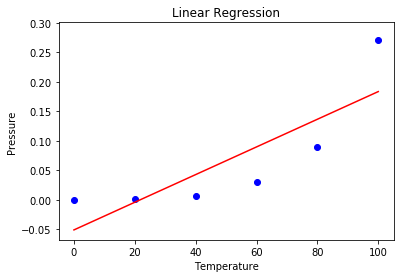
\includegraphics[scale=0.6]{assets/polynomial_straight_line.png}
    \caption{Non-linear relationship}
\end{figure}

In that case, we are stuck with a straight line that cannot fit the data points properly.
In this example, what if we could express $y$ not as a function of $x$, but also of $x^2$, and maybe even $x^3$ and $x^4$?
We could make a hypothesis that draws a nice \textbf{curve} that would better fit the data.
That's where polynomial features can help!

% =============================================== %
\section*{Interlude - Polynomial features}
% ----------------------------------------------- %
First we get to do some \textit{feature engineering}.
We create new features by raising our initial $x$ feature to the power of 2, and then 3, 4... as far as we want to go.
For each new feature we need to create a new column in the dataset.

% =============================================== %
\section*{Interlude - Polynomial Hypothesis}
% ----------------------------------------------- %
Now that we created our new features, we can combine them in a linear hypothesis that looks just the same as what we're used to:

$$
\hat{y} = \theta_0 + \theta_1 x  +\theta_2 x^{2} + \dots + \theta_n x^{n}
$$  

It's a little strange because we are building a linear combination, not with different features but with different powers of the same feature.
This is a first way of introducing non-linearity in a regression model!